\documentclass[12pt]{article}

\usepackage{amsmath, amsfonts, bm, graphicx}
\usepackage{tabularx}
\usepackage{booktabs} 
\usepackage{float}

\title{Ph291E Lab 2 -- Index of Refraction}
\author{
    Zeshui Song\\
    The Cooper Union
}
\date{September 25, 2025}

\begin{document}

\maketitle

\section{Purpose}  
In this lab, Pfund's method and Snell's law was used to determine the index of refraction of an unknown liquid. Additionally, error analysis and calculation of error propagation were performed to compare the experimental results with the known value of the index of refraction for the liquid. 

\section{Data}
\paragraph{Part A: Pfund's Method} \mbox{}\\
% Petri Dish Thickness
\begin{table}[H]
\centering
\caption{Petri Dish Thickness}
\scriptsize 
\begin{tabular}{ccccc}
\toprule
\textbf{Thickness (mm)} & \textbf{Inst. Error (mm)} & \textbf{Random Error (mm)} \\
\midrule
2.180 & & \\
2.190 & & \\
2.185 & & \\
2.185 & & \\
2.195 & & \\
2.180 & 0.005 & 0.002 \\
\midrule
\multicolumn{3}{l}{\textbf{Mean Thickness}} & \multicolumn{2}{l}{\textbf{2.186 mm}} \\
\bottomrule
\end{tabular}
\end{table}

% Ring Diameter Without Liquid			
\begin{table}[H]
\centering
\caption{Ring Diameter Without Liquid}
\scriptsize 
\begin{tabular}{ccccc}
\toprule
\textbf{Diameter (mm)} & \textbf{Inst. Error (mm)} & \textbf{Random Error (mm)} \\
\midrule
7.78 & & \\
7.74 & & \\
7.68 & & \\
7.70 & &  \\
7.66 & & \\
7.40 & 0.02 & 0.05\\
\midrule
\multicolumn{3}{l}{\textbf{Mean Diameter}} & \multicolumn{2}{l}{\textbf{7.66 mm}} \\
\bottomrule
\end{tabular}
\end{table}

% Ring Diameter With Liquid			
\begin{table}[H]
\centering
\caption{Ring Diameter With Liquid}
\scriptsize 
\begin{tabular}{ccccc}
\toprule
\textbf{Diameter (mm)} & \textbf{Inst. Error (mm)} & \textbf{Random Error (mm)} \\
\midrule
16.30 & & \\
16.12 & & \\
15.98 & & \\
15.62 & & \\
15.30 & & \\
15.72 &0.02 &0.14 \\
\midrule
\multicolumn{3}{l}{\textbf{Mean Diameter}} & \multicolumn{2}{l}{\textbf{15.84 mm}} \\
\bottomrule
\end{tabular}
\end{table}

\paragraph{Part B: Snell's Law} \mbox{}\\
% Snell's Law		
\begin{table}[H]
\centering
\caption{Snell's Law Measurements for $\theta_1$ and $\theta_2$}
\scriptsize 
\begin{tabular}{ccccc}
\toprule
\textbf{Incident Angle (deg)} & \textbf{Refracted Angle (deg)} & \textbf{Inst. Error (deg)} \\
\midrule
48.0 & 33.0& \\
54.0 & 33.0 & \\
33.0 & 25.0 & 0.5\\
\bottomrule
\end{tabular}
\end{table}

\begin{table}[H]
\centering
\caption{Snell's Law Measurements for $\theta_3$ and $\theta_4$}
\scriptsize 
\begin{tabular}{ccccc}
\toprule
\textbf{Incident Angle (deg)} & \textbf{Refracted Angle (deg)} & \textbf{Inst. Error (deg)} \\
\midrule
35.0 & 45.0 & \\
33.0 & 34.0 & \\
23.0 & 32.0 & 0.5\\
\bottomrule
\end{tabular}
\end{table}

\newpage
\section{Calculations}
\paragraph{Petri Dish Thickness Sample Calculations} \mbox{}\\
\textbf{Mean Calculation:}
\[\bar{x} = \frac{1}{n} \sum_{i=1}^{n} x_i\]
\[\bar{x} = \frac{1}{6} (2.180+2.190+2.185+2.185+2.195+2.180)\]
\[\bar{x} =  \text{2.1858 mm}\]
\textbf{Standard Deviation:}
\[S_x = \sqrt{\frac{1}{n-1} \sum_{i=1}^{n} (x_i - \bar{x})^2}\]
\[
\begin{aligned}
S_x &= \sqrt{\frac{1}{6-1} \Big[ (2.180-2.1858)^2 + (2.190-2.1858)^2 + \cdots + (2.180-2.1858)^2 \Big]} \\
\end{aligned}
\]
\[S_x =  \text{0.005845 mm}\]
\textbf{Standard Deviation of the Mean (SDOM):}
\[\sigma_{\bar{x}} = \frac{S_x}{\sqrt{n}}\]
\[\sigma_{\bar{x}} = \frac{0.005845}{\sqrt{6}}\]
\[\sigma_{\bar{x}}=  \text{0.0023863 mm}\]
The same procedure was applied to calculate the mean, standard deviation and standard deviation of the mean for the remaining measurements.
\paragraph{Pfund's Method and Error Propagation} \mbox{}\\
\textbf{Index of Refraction of Glass:}
\[n_{glass} = \frac{\sqrt{d^2+16t^2}}{d}\]
\[n_{glass} = \frac{\sqrt{(7.66)^2+16(2.18583)^2}}{(7.66)}\]
\[n_{glass} = 1.51751\]
\textbf{Error Propagation for $n_{glass}$:}
\[\delta_{n_{glass}} = \left|\frac{\partial n_{glass}}{\partial d}\delta_d\right| + \left|\frac{\partial n_{glass}}{\partial t}\delta_t\right|\]
Since the measurement of the diameter depends on the thickness of the glass, small variations in thickness at different points can cause the diameter to change. Thus, the error propagation is performed using the absolute sum method.
\[\frac{\partial n_{glass}}{\partial d} = -\frac{16t^2}{d^2\sqrt{d^2+16t^2}}, \quad \frac{\partial n_{glass}}{\partial t} = \frac{16t}{d\sqrt{d^2+16t^2}}\]
\textbf{Chosen uncertainties:} $\delta d = 0.05~\mathrm{mm}$ (random, larger than instrumental) and $\delta t = 0.005~\mathrm{mm}$ (instrumental, larger than random).
\[
\delta_{n_{glass}} =   \left|-\frac{16t^2}{d^2\sqrt{d^2+16t^2}}\delta_d\right| + \left|\frac{16t}{d\sqrt{d^2+16t^2}}\delta_t\right|\]
\\
\[\delta_{n_{glass}} = |A|+|B|\]
\[where \quad A = -\frac{16t^2}{d^2\sqrt{d^2+16t^2}}\delta_d, \quad B=\frac{16t}{d\sqrt{d^2+16t^2}}\delta_t\]
\[A=-\frac{16(2.18583)^2}{(7.66)^2 \sqrt{(7.66)^2 + 16(2.18583)^2}} (0.05) = -0.006152\] 
\[B=\frac{16(2.18583)}{7.66 \sqrt{(7.66)^2 + 16(2.18583)^2}} (0.005)= 0.0019638\]
\[\delta_{n_{glass}} = |-0.006152|+|0.0019638|\]
\[\delta_{n_{glass}} = 0.0081164\]
\textbf{Index of Refraction of Unknown Liquid:}
\[n_{liquid} = \frac{n_{glass}d_l}{\sqrt{d_l^2+16t^2}}\]
\[n_{liquid} = \frac{(1.51751)(15.84)}{\sqrt{(15.84)^2+16(2.18583)^2}}\]
\[n_{liquid} = 1.32856\]
\textbf{Error Propagation for $n_{liquid}$:}
\[
\delta_{n_{liquid}} = 
\left| \frac{\partial n_{liquid}}{\partial n_{glass}}\delta_{n_{glass}} \right| +
\left| \frac{\partial n_{liquid}}{\partial d_l} \delta_{d_l} \right| +
\left| \frac{\partial n_{liquid}}{\partial t}\delta_t \right|
\]
Since the calculation of $n_{liquid}$ depends on the previously calculated value of $n_{glass}$ as well as the Petri dish thickness, these uncertainties are dependent. Therefore, the error propagation is carried out using the absolute sum method.
\[\frac{\partial n_{liquid}}{\partial n_{glass}} = \frac{d_l}{\sqrt{d_l^2+16t^2}}, \quad \frac{\partial n_{liquid}}{\partial d_l} = \frac{16t^2 n_{glass}}{(d_l^2+16t^2)^{3/2}}, \quad \frac{\partial n_{liquid}}{\partial t} = -\frac{16t d_l n_{glass}}{(d_l^2+16t^2)^{3/2}}\]
\textbf{Chosen uncertainties:} $\delta_{n_glass} = 0.006~\mathrm{mm}$ (calculated), $\delta d_l = 0.14~\mathrm{mm}$ (random, larger than instrumental) and $\delta t = 0.005~\mathrm{mm}$ (instrumental, larger than random).
\[
\delta_{n_{liquid}} = 
\left| \frac{d_l}{\sqrt{d_l^2+16t^2}} \delta_{n_{glass}} \right| +
\left| \frac{16t^2 n_{glass}}{(d_l^2+16t^2)^{3/2}} \delta_{d_l} \right| +
\left| -\frac{16t d_l n_{glass}}{(d_l^2+16t^2)^{3/2}} \delta_t \right|
\]
\[\delta_{n_liquid}= |A| + |B| + |C|\]
\[where \quad A = \frac{d_l}{\sqrt{d_l^2+16t^2}} \delta_{n_{glass}}, \quad B = \frac{16t^2 n_{glass}}{(d_l^2+16t^2)^{3/2}} \delta_{d_l}, \quad C = -\frac{16t d_l n_{glass}}{(d_l^2+16t^2)^{3/2}} \delta_t\]

\[A = \frac{15.84}{\sqrt{15.84^2 + 16(2.18583)^2}} (0.0081164)=0.007105\]
\[B = \frac{16(2.18583)^2 (1.51751)}{(15.84^2 + 16(2.18583)^2)^{3/2}} (0.14877)=0.001075\]
\[C = -\frac{16(2.18583)(15.84)(1.51751)}{(15.84^2 + 16(2.18583)^2)^{3/2}} (0.005)=-0.0007096\]
\[\delta_{n_liquid}= |0.007105| + |0.001075| + |-0.0007096|\]
\[\delta_{n_liquid}= 0.0.00889\]

\paragraph{Snell's Law and Error Propagation for $\theta_1$ and $\theta_2$ (First Interface)} \mbox{}\\
\[n_{air}sin(\theta_1)=n_{liquid}sin(\theta_2) \]
\[n_{liquid} = \frac{n_{air}sin(\theta_1)}{sin(\theta_2)} \quad (n_{air} \approx 1)\]
\[n_{liquid} = \frac{sin(48^\circ)}{sin(33^\circ)}\]
\[n_{liquid} = 1.36447221\]
\textbf{Error Propagation for $n_{liquid}$:}
\[\delta_{n_{liquid}} = \left | \frac{\partial n_{liquid}}{\partial \theta_1}\delta_{\theta_1} \right |+ \left | \frac{\partial n_{liquid}}{\partial \theta_2}\delta_{\theta_2} \right |\]
Since the measurement of the angles are dependent on the placement of the center of the circle, which was done by constructing the perpendicular bisectors of two chords, the error propagation is carried out using the absolute sum method.
\[\frac{\partial n_{liquid}}{\partial \theta_1} = \frac{n_{air}cos(\theta_1)}{sin(\theta_2)}, \quad \frac{\partial n_{liquid}}{\partial \theta_2} = -\frac{n_{air}sin(\theta_1)cos(\theta_2)}{sin^2(\theta_2)}\]
\textbf{Chosen uncertainties:} $\delta_{\theta_1} = \delta_{\theta_2} = 0.5~\mathrm{deg}$ (instrumental).
\[\delta_{n_{liquid}} = \left|\frac{n_{air}cos(\theta_1)}{sin(\theta_2)} \delta_{\theta_1}\right| + \left| -\frac{n_{air}sin(\theta_1)cos(\theta_2)}{sin^2(\theta_2)} \delta_{\theta_2}\right| \quad (n_{air} \approx 1)\]
\[\delta_{n_{liquid}} = \left|\frac{cos(48^\circ)}{sin(33^\circ)} \left (0.5^\circ \frac{\pi}{180}\right )\right| + \left| -\frac{sin(48^\circ)cos(33^\circ)}{sin^2(33^\circ)} \left (0.5^\circ \frac{\pi}{180}\right )\right|\]
$\delta_{\theta_1}$ and $\delta_{\theta_2}$ are converted from degrees to radians for the calculation.
\[\delta_{n_{liquid}} = 0.02905\]
This calculation was repeated for each of the 3 angles of incidence for 3 values of the index of refraction of the unknown liquid.

\paragraph{Snell's Law and Error Propagation for $\theta_3$ and $\theta_4$ (Second Interface)} \mbox{}\\
\[n_{liquid}sin(\theta_3)=n_{air}sin(\theta_4) \]
\[n_{liquid} = \frac{n_{air}sin(\theta_4)}{sin(\theta_3)} \quad (n_{air} \approx 1)\]
\[n_{liquid} = \frac{sin(45^\circ)}{sin(35^\circ)}\]
\[n_{liquid} = 1.23280\]
\textbf{Error Propagation for $n_{liquid}$:}
\[\delta_{n_{liquid}} = \left | \frac{\partial n_{liquid}}{\partial \theta_3}\delta_{\theta_3} \right |+ \left | \frac{\partial n_{liquid}}{\partial \theta_4}\delta_{\theta_4} \right |\]
Since the measurement of the angles are dependent on the placement of the center of the circle, which was done by constructing the perpendicular bisectors of two chords, the error propagation is carried out using the absolute sum method.
\[\frac{\partial n_{liquid}}{\partial \theta_3} = -\frac{n_{air}sin(\theta_4)cos(\theta_3)}{sin^2(\theta_3)}, \quad \frac{\partial n_{liquid}}{\partial \theta_4} =\frac{n_{air}cos(\theta_4)}{sin(\theta_3)} \]
\textbf{Chosen uncertainties:} $\delta_{\theta_3} = \delta_{\theta_4} = 0.5~\mathrm{deg}$ (instrumental).
\[\delta_{n_{liquid}} = \left|-\frac{n_{air}sin(\theta_4)cos(\theta_3)}{sin^2(\theta_3)}\delta_{\theta_3}\right| + \left|\frac{n_{air}cos(\theta_4)}{sin(\theta_3)}\delta_{\theta_4} \right| \quad (n_{air} \approx 1)\]
\[\delta_{n_{liquid}} = \left|-\frac{sin(45^\circ)cos(35^\circ)}{sin^2(35^\circ)}\left(0.5^\circ \frac{\pi}{180}\right)\right| + \left|\frac{cos(45^\circ)}{sin(35^\circ)}\left(0.5^\circ \frac{\pi}{180}\right) \right|\]


$\delta_{\theta_3}$ and $\delta_{\theta_4}$ are converted from degrees to radians for the calculation.
\[\delta_{n_{liquid}} = 0.026122\]
This calculation was repeated for each of the 3 angles of incidence for 3 values of the index of refraction of the unknown liquid.\\  \\


\section{Error Analysis}
\paragraph{Pfund's Method} \mbox{}\\
Looking at the error propogation for $n_{glass}$, the term $A$ which depended on $\delta_d$ contributed more to the overall uncertainty than term $B$ which depended on $\delta_t$. This reflects the fact that random error in the diameter measurement was larger than the instrumental error in the thickness measurement. It is likely that some systematic error may have been introduced in the measurement of the ring diameters due to estimating the edges of the rings and measuring the diameters from the center instead of a well defined line, while the thickness showed less variation since it was measured near the Petri dish edges where it is more uniform. Similarly, for the error propogation of $n_{liquid}$, term $A$ which depended on the uncertainty in $n_{glass}$ contributed the most to the overall uncertainty, since it includes the propogated from the first diameter and thickness measurements.

\paragraph{Snell's Law} \mbox{}\\
The values of $n_{liquid}$ ranged from 1.0 to 1.5 which do not agree within their error bars. This large spread in values is likely due to systematic errors such as the misplacement of the center of the circle when measuring the angles of incidence and refraction and not placing the pins exactly on the laser path, causing inaccurate angle measurements. Additionally, by placing the pins A,B,C and D further apart, it minimizes the uncertainty in the angle measurements such that it is less than the instrumental error from the protractor.\\
The values of $n_{liquid}$ calculated from Snell's law along with their uncertainties are shown below:
\begin{align*}
n_{\text{liquid}} &= 1.4 \pm 0.03 \\
n_{\text{liquid}} &= 1.5 \pm 0.03 \\
n_{\text{liquid}} &= 1.3 \pm 0.04 \\
n_{\text{liquid}} &= 1.2 \pm 0.03 \\
n_{\text{liquid}} &= 1.0 \pm 0.03 \\
n_{\text{liquid}} &= 1.4 \pm 0.05
\end{align*}
The average and standard deviation of the mean of these values were calculated to be:
\[\bar{n}_{liquid} = 1.3 \pm 0.06\]
Out of the range of uncertainties, the SDOM is the largest and was chosen as the uncertainty for the average value. This reflects the large spread in values calculated from Snell's law and that the uncertainty was mainly composed of systematic errors.


\section{Results}
\paragraph{Pfund's Method:} \mbox{}
\begin{align*}
\text{Index of Refraction of Glass:} \quad & n_{\text{glass}} = 1.52 \pm 0.008 \\
\text{Index of Refraction of Unknown Liquid:} \quad & n_{\text{liquid}} = 1.32 \pm 0.009
\end{align*}

\paragraph{Snell's Law:} \mbox{}\\
\[\text{Index of Refraction of Unknown Liquid:} \quad \bar{n}_{\text{liquid}} = 1.3 \pm 0.06\]

\section{Conclusion}
Both Pfund's method and Snell's law were able to determine the index of refraction of the unknown liquid (later revealed to be tap water) and both results agreed with the actual value of approximately 1.33 within their error bars. However, Pfund's method yielded a more precise result with a smaller uncertainty (0.009) compared to Snell's law (0.06). This is likely due to the systematic errors previously discussed introducing uncertainty in the angle measurements for Snell's law which was much more significant than the random and instrumental errors for Pfund's method. \\ \\
A comparison of the results from Pfund's method and Snell's law along with the actual value of the index of refraction of tap water (1.33) is shown below:
\begin{figure}[H]
    \centering
    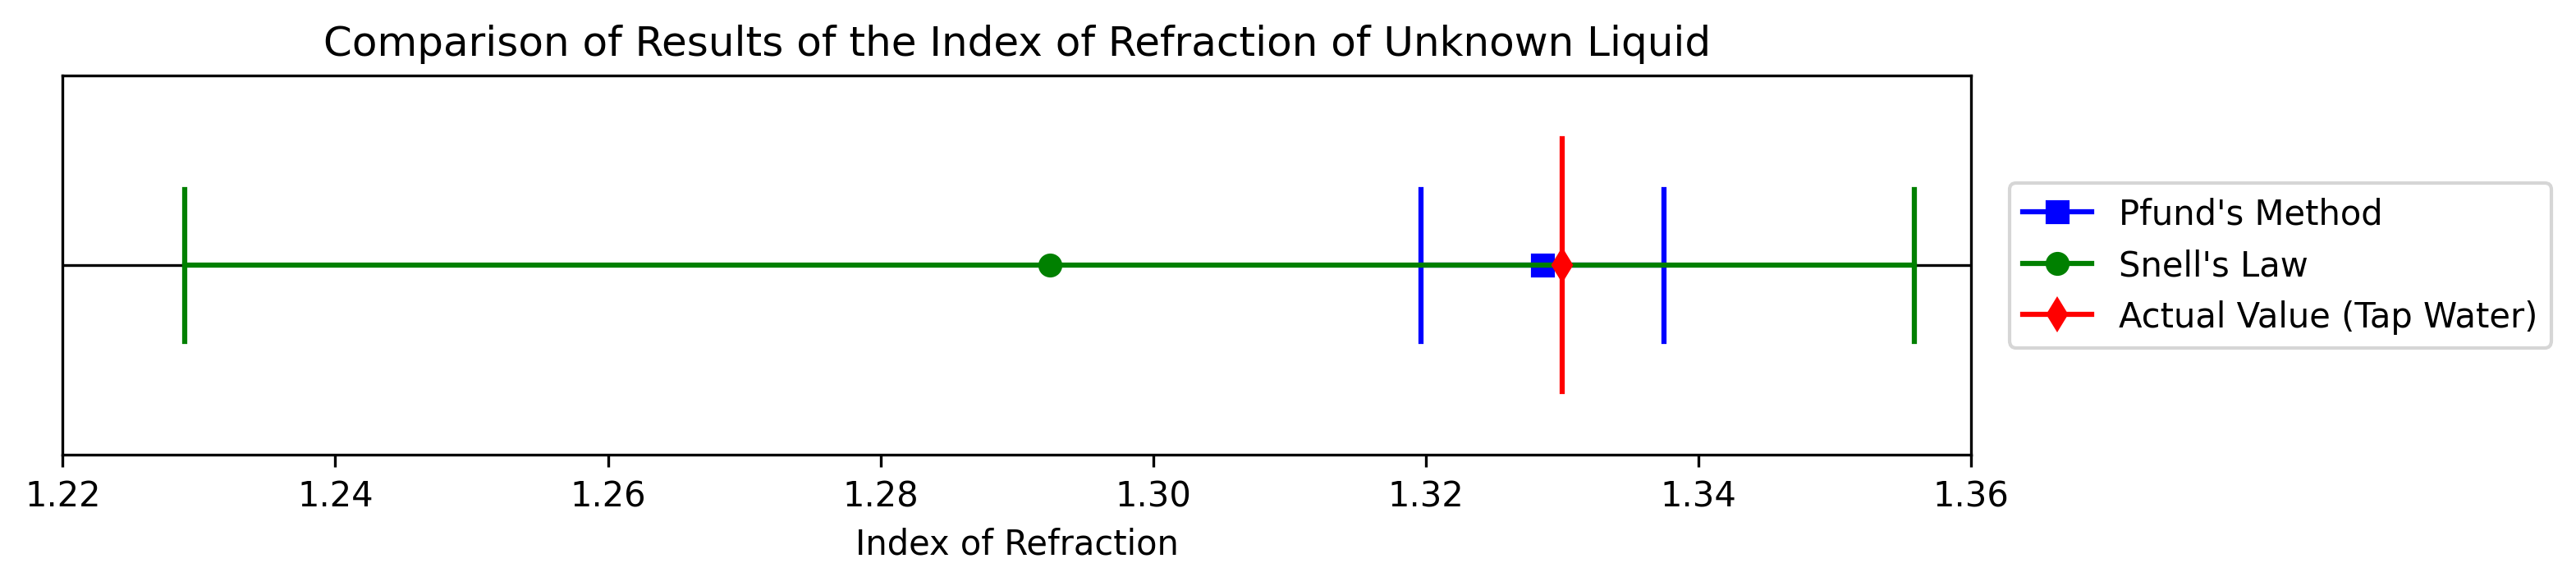
\includegraphics[width=1\textwidth]{results.png}
\end{figure}
Overall, Pfund's method proved to be a more reliable and accurate method for determining the index of refraction of the unknown liquid in this experiment.

\newpage
\section{Answers to questions}
\paragraph{Question 1} \mbox{}\\
\begin{figure}[H]
    \centering
    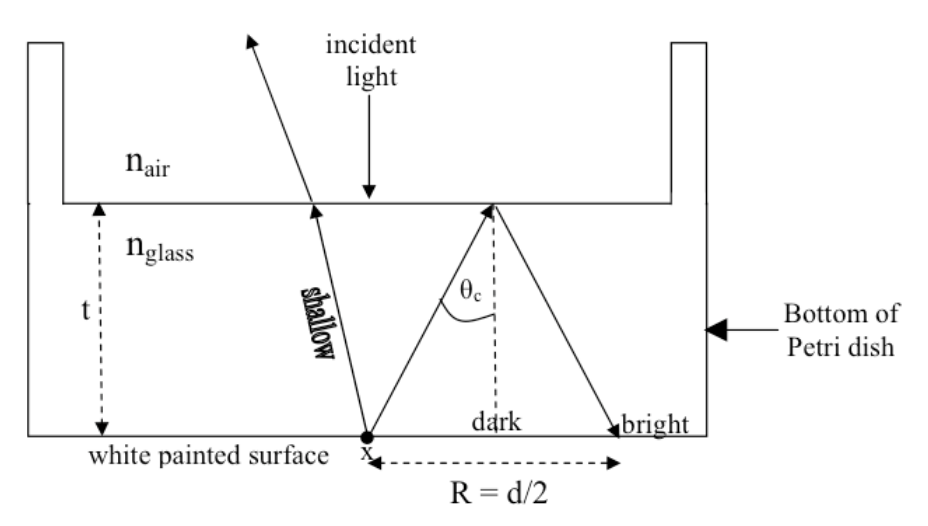
\includegraphics[width=0.7\textwidth]{1.png}
\end{figure}
\[sin(\theta_c)=\frac{n_{air}}{n_{glass}} \quad (\text{$n_{air}$ is approximately 1})\]
\[n_{glass}=\frac{1}{sin(\theta_c)}\]
\[sin(\theta_c)=\frac{d/4}{\sqrt{(d/4)^2+t^2}}=\frac{d}{\sqrt{d^2+16t^2}}\]
\[n_{glass}=\frac{\sqrt{d^2+16t^2}}{d}\]
\newpage
\paragraph{Question 2} \mbox{}\\
\begin{figure}[H]
    \centering
    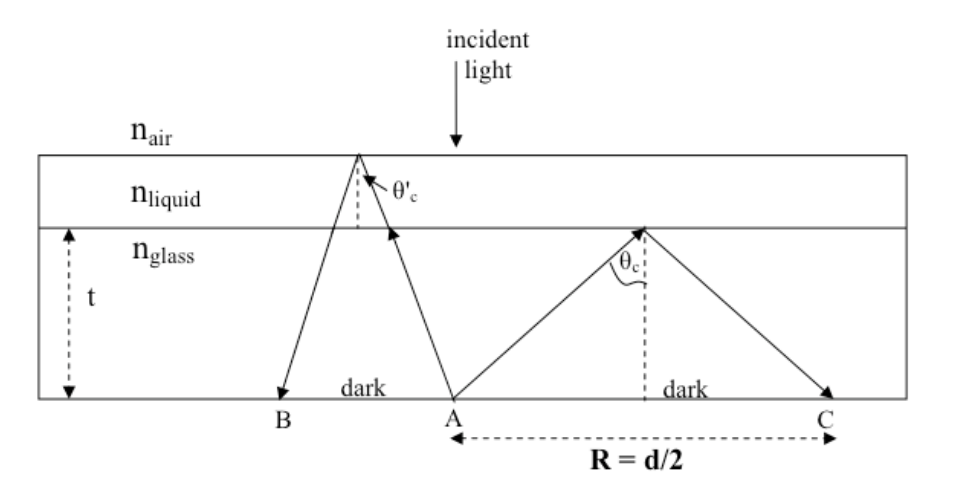
\includegraphics[width=0.7\textwidth]{2.png}
\end{figure}
\[sin(\theta_c)=\frac{n_{liquid}}{n_{glass}}\]
\[n_{liquid}=n_{glass}sin(\theta_c)\]
\[sin(\theta_c)=\frac{d/4}{\sqrt{(d/4)^2+t^2}}=\frac{d}{\sqrt{d^2+16t^2}}\]
\[n_{liquid}=\frac{n_{glass}d}{\sqrt{d^2+16t^2}}\]
\paragraph{Question 3} \mbox{}\\
It was assumed that the laser path followed the straight line between pins A and B and between pins C and D, and that the ray intersected the petri dish exactly at the points where the traced lines intersected. It was also assumed that the line drawn from the center of the petri dish to the point of intersection was normal to the surface of the petri dish. These assumptions may not be fully reasonable since it introduced signficant systematic error, shown by the SDOM in $n_{liquid}$ being 0.06. An additional assumption made was that $n{air} \approx 1$, which is reasonable since the index of refraction of air is very close to 1.
\paragraph{Question 4} \mbox{}\\
Since Pfund's method is based on the physics of total internal reflection, it won't work for liquids of all n. The critical angle is related to the index of refraction by $sin(\theta_c) = n_{liquid}/n_{glass}$, the ratio of $n_{liquid}/n_{glass}$ must be less than 1. Thus, the index of refraction of the liquid must be less than that of the glass.
\end{document}
